In an effort to help researchers glean insight from tweets, Twitter offers
a streaming API that streams all tweets that contain a certain string.
We leverage this service to gather data surrounding the popular television
show The Walking Dead and then measure the number of tweets that occur in a given
hour over a time span.

Using the programming language Python and the library tweepy, a popular
wrapper for the Twitter streaming API, we collected all tweets containing the
hashtag ``\#thewalkingdead'' for three weeks from 2015-11-07 21:00 EST to
2015-11-23 21:00 EST. As this television show airs Sundays at 21:00 EST,
of particular importance is the tweets occurring around this time.
We therefore restrict our measurements to 24 hours prior to and 24 hours after
the television show's airing for the above three week time frame.

These measurements give rise to the timeseries presented in Figure \ref{tweets_plot}

\begin{figure}[!T]
  \centerline{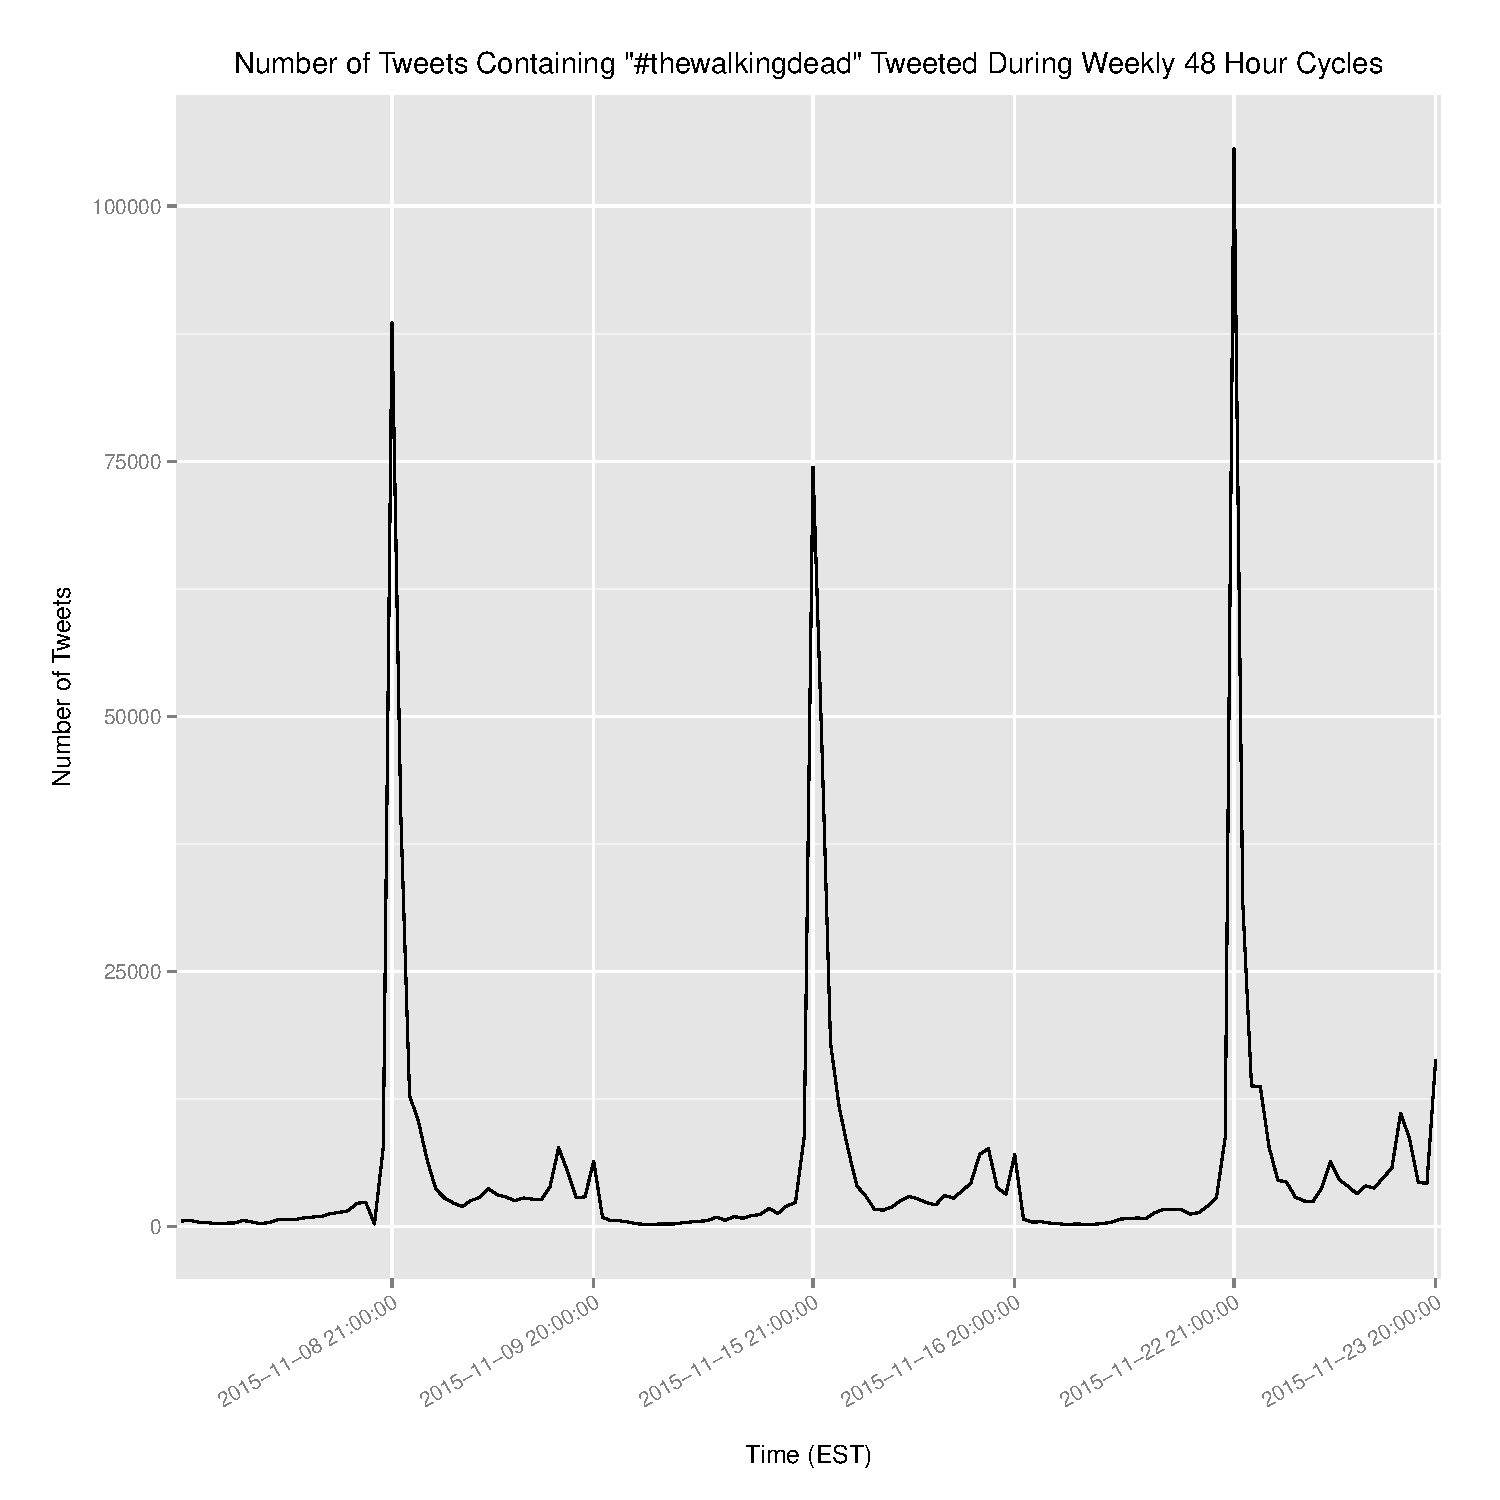
\includegraphics{../analysis/plots/tweets_plot}}
  \caption{Time series plot of number of tweets containing the hashtag
  \#thewalkingdead over three 48 hour cycles.}\label{tweets_plot}
\end{figure}
